\documentclass[a4paper,openright,12pt]{report}
\usepackage[spanish]{babel}			% Permite que partes automáticas del documento aparezcan en castellano.
\usepackage[utf8]{inputenc}			% Permite escribir tildes y otros caracteres directamente en el .tex
\usepackage[T1]{fontenc}   		         % Asegura que el documento resultante use caracteres de una fuente
\usepackage{listings}				% Permite utilizar lenguajes de programacion dentro de latex
\usepackage{enumerate}				%enumerados
\usepackage{graphicx}%graficos

\begin{document}

\begin{titlepage}

\begin{center}
\vspace*{-1in}
\begin{figure}[htb]
\begin{center}

\includegraphics[width=8cm]{./imagenes/espol.jpg}
\end{center}
\end{figure}
FACULTAD DE INGENIERIA EN ELECTRICIDAD Y COMPUTACIÓN\\
\vspace*{0.15in}
LENGUAJES DE PROGRAMACIÓN\\
\vspace*{0.6in}
\begin{large}
PROYECTO DE SEGUNDO PARCIAL: PYTHON
\end{large}
\vspace*{0.4in}
\begin{large}
ANALIZADOR SINTÁCTICO DE UN ARCHIVO XML\\
\end{large}
\vspace*{0.3in}
\rule{80mm}{0.1mm}\\
\vspace*{0.1in}
\begin{large}
Integrantes:\\Leonel Ramírez Gonzalez\\José Vélez Gómez\\Kevin Campuzano Castillo\\ 
\end{large}
\end{center}
\end{titlepage}

\tableofcontents
\chapter{Objetivos}
\begin{itemize}
\item{Comprender, entender e implementar la sintaxis del Lenguaje de programacion Python.}
\item{Ventajas y Desventajas del lenguaje de programacion Python referente a otros lenguajes.}
\item{Implementar clases en Python.}
\item{Sacar ventaja de este lenguaje que es multiparadigma.}
\end{itemize}

\chapter{Introducción}
\begin{figure}[htb]
\begin{center}

\includegraphics[width=8cm]{./imagenes/Python_Logo.png}
\end{center}
\end{figure}
\textbf{Python} es un lenguaje de programación creado por Guido van Rossum a finales de los ochenta, y que gracias a sus características ha llegado a ser un lenguaje muy conocido en la actualidad.
Python es un lenguaje muy simple, por lo que es muy fácil iniciarse en este lenguaje. El pseudo-código natural de Python es una de sus grandes fortalezas.\\

Usando el lenguaje Python se puede crear todo tipo de programas; programas de propósito general y también se pueden desarrollar páginas Web.\\

Python contiene una gran cantidad de librerías, tipos de datos y funciones incorporadas en el propio lenguaje, que ayudan a realizar muchas tareas comunes sin necesidad de tener que programarlas desde cero.\\
Las librerías pueden ayudar a hacer varias cosas como expresiones regulares, generación de documentos, evaluación de unidades, pruebas, procesos, bases de datos, navegadores web, CGI, ftp, correo electrónico, XML, XML-RPC, HTML, archivos WAV, criptografía, GUI, y también otras funciones dependientes del Sistema.\\

Python tiene una sintaxis muy visual, gracias a que maneja una sintaxis identada (con márgenes), que es de caracter obligatorio. Para separar los bloques de código en Python se debe tabular hacia dentro. Esto ayuda a que todos los programadores adopten las mismas notaciones y que los programas hechos en Python tengan un aspecto muy similar.\\


\chapter{Alcance del Proyecto}
Se investigo la manera de hacer parseo que es basicamente analizar una estructura de simbolos con el objetivo de terminar su estructura gramatica, como el
caso de un archivo XML, generalmente un parseo, primero identifica los simbolos de entrada y luego lo va transformando 
a una estructura mas fácil de entender generalmente un arbol pero en nuestro caso se transforma en una lista de estructura de datos.\\

Para armar la estructura en Python, se investigo desde la pagina fuente, que es la pagina de la organización Python en la que nos demuestra que las estructuras son clases y se las implementa de la siguiente manera con sus respectivas funciones getter y setter.\\\\\\\\

\lstset{language=Python}          % Set your language (you can change the language for each code-block optionally)
Estructura de la clase Device
\begin{lstlisting}[frame=single]  % Start your code-block
class Device:
    def __init__(self, idD, user_agent, fall_back):
        self.idD = idD
        self.user_agent = user_agent
        self.fall_back = fall_back

   def setDevice(self, lista):
        idD, ug, fb, *listD = lista
        self.idD = idD
        self.user_agent = ug
        self.fall_back = fb
    def getIdDevice(self):
        return self.idD
    def setIdDevice(self, idD):
        self.idD = idD
    def getUserAgentDevice(self):
        return self.user_agent
    def setUserAgentDevice(self, user_agent):
        self.user_agent = user_agent
    def getFallBackDevice(self):
        return self.fall_back
    def setFallBackDevice(self, fall_back):
        self.fall_back = fall_back
\end{lstlisting}

Estructura de la clase Group
\begin{lstlisting}[frame=single]  % Start your code-block
class Group:
    def __init__(self, idG):
        self.idG = idG

    def setGroup(self, lista):
        idG, *list = lista
        self.idG = idG
    def getIdGroup(self):
        return self.idG
    def setIdGroup(self, idG):
        self.idG = idG
\end{lstlisting}

Estructura de la clase Capability
\begin{lstlisting}[frame=single]  % Start your code-block
class Capability:
    def __init__(self, name, value):
        self.name = name
        self.value = value

    def setCapability(self, listaC):
        name, value,*list = listaC
        self.name = name
        self.value = value
    def getNameCapability(self):
        return self.name
    def setNameCapability(self, name):
        self.name = name
    def getValueCapability(self):
        return self.value
    def setValueCapability(self, value):
        self.value = value
\end{lstlisting}

Esto graficamente se representa como se lo muestra en la figura 1.1, en la cual nosotros decidimos separarlos cada uno por su estructura,en esta parte se tuvo problemas con la decision de como serian las estructuras de los grupos por ciertas correcciones que se hicieron con este proyecto en base a nuevas especificaciones de nuestro profesor. Se lo hizo de esta manera por que no vimos la necesidad de que estuviera asi ya que no lo almacenariamos en un archivo sino que solamente se lo procesaria en el mismo momento en que se forman su estructura.\\
\begin{figure}[htbp]
	\begin{center}
		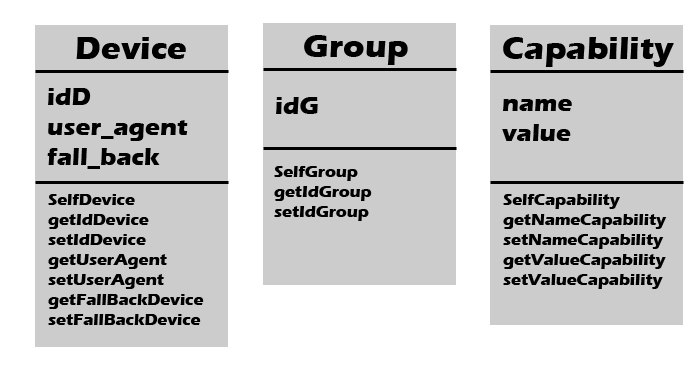
\includegraphics[width=.90\textwidth]{./imagenes/estructuras_python.jpg}
		\caption{Estructura de datos}
		\label{Estructura de datos}
	\end{center}
\end{figure}

Al archivo Xml se le hizo algunos pasos para poder llegar al punto que deseamos. Traducimos las funciones que creamos en
el programa de Haskell al lenguaje de programación Python, por una parte se hizo mas sencillo ya que Python es un lenguaje 
sencillo, limpio tuvimos que recurrir a otros metodos ya que ciertas funciones no se encontraban en Python. 

\chapter{Observaciones}
\begin{itemize}
\item \textbf{Leonel Ramírez Gonzalez}
\begin{itemize}
	\item[Ventajas: ]fácil de implementar variables, no se necesita declarar el tipo de variable.
python se encarga de eso.
	\item[Desventajas: ]La desventaja que encontre es que no se puede usar recursividad con archivos demasiados grandes por que python utiliza colas y estas se pueden llenar a su limite por lo tanto votara un error.
\end{itemize}
\item \textbf{José Vélez Gómez}
\begin{itemize}
	\item[Ventajas: ]Existe gran cantidad de funciones y librerías. Sencillo y rápido de programar.
	\item[Desventajas: ]Oculta el uso de memoria.Los programas interpretados son mas lentos que los compilados.Sin
embargo los programas interpretados suelen ser cortos, en los que la diferencia es inapreciable.
\end{itemize}
\item \textbf{Kevin Campuzano Castillo}
\begin{itemize}
	\item[Ventajas: ]Python es un lenguaje limpio para programar. Permite la creación de todo tipo de programas incluyendo sitios web.
	\item[Desventajas: ] lentitud por ser un lenguaje interpretado.
\end{itemize}
\end{itemize}
\end{document}